%\vspace{-2ex}
\section{Introduction} \label{sec:intro}

%Various tools have been proposed which do different things
In recent years, there has been a tremendous amount of activity in executable-level research targeting varied applications like security vulnerability analysis~\cite{Brumley-Mayhem,Song-Bitblaze}, bug testing~\cite{Chipounov-S2E}, and binary optimizations~\cite{plto, ispike}. In spite of a significant overlap in the overall goals of various source-code methods and executables-level techniques, several analyses and sophisticated transformations that are well-understood and implemented in source-level infrastructures have yet to become available in binary frameworks. Many of the executable-level tools suggest new techniques for performing elementary source-level tasks. For example, PLTO~\cite{plto} proposes a custom alias analysis technique to implement a simple transformation like constant propagation in executables. Similarly, several techniques for detecting security vulnerabilities in source code~\cite{Wagner-afirst, Bush-static} remain outside the realm of current executable level frameworks. 

%in spite of overlapping of some methods, lots of thse tools suggest new theory,, bandera-extracting
%Example of binary and source tools which achieve same tasks but are based on different foundations. 
%SymExection - read if bitblaze has dynamic sym exection
%and various tools have been suggested to perform different tasks on executables 
%The reason for the great interest in executable-level tools is that they offers many additional advantages over traditional source-level frameworks: these tools enable the analysis and transformations in the absence of source code, thereby extending their applicability to commercial off-the shelf components and legacy binaries and can also be employed by an end-user to embed custom security enforcements and perform platform specific customizations.
%
It is a well known fact that a standalone binary without any metadata is less amenable to analysis than the source code. \emph{However, we believe that one of the prime reason why current binary frameworks resort to devising new techniques is that these frameworks define their own low-level intermediate representations (IR) which are significantly more constrained than an IR used in a source-code framework}. IRs used in existing binary frameworks lack high level features like an abstract stack, symbols and are machine dependent in some cases. This severely limits the application of source-level analyses to binaries and necessitates new research to make them applicable. We convert the binaries to the same high-level IR that compilers use, enabling the application of source-level research to executables.

We have integrated our techniques in a prototype x86 binary framework called SecondWrite that uses LLVM, a widely-used compiler infrastructure, as IR. Our framework has the following main applications:


\begin{figure*}[t]
{
%\vspace{-0.2in}
%\centering
\begin{minipage}{.58\linewidth}
\centering
{
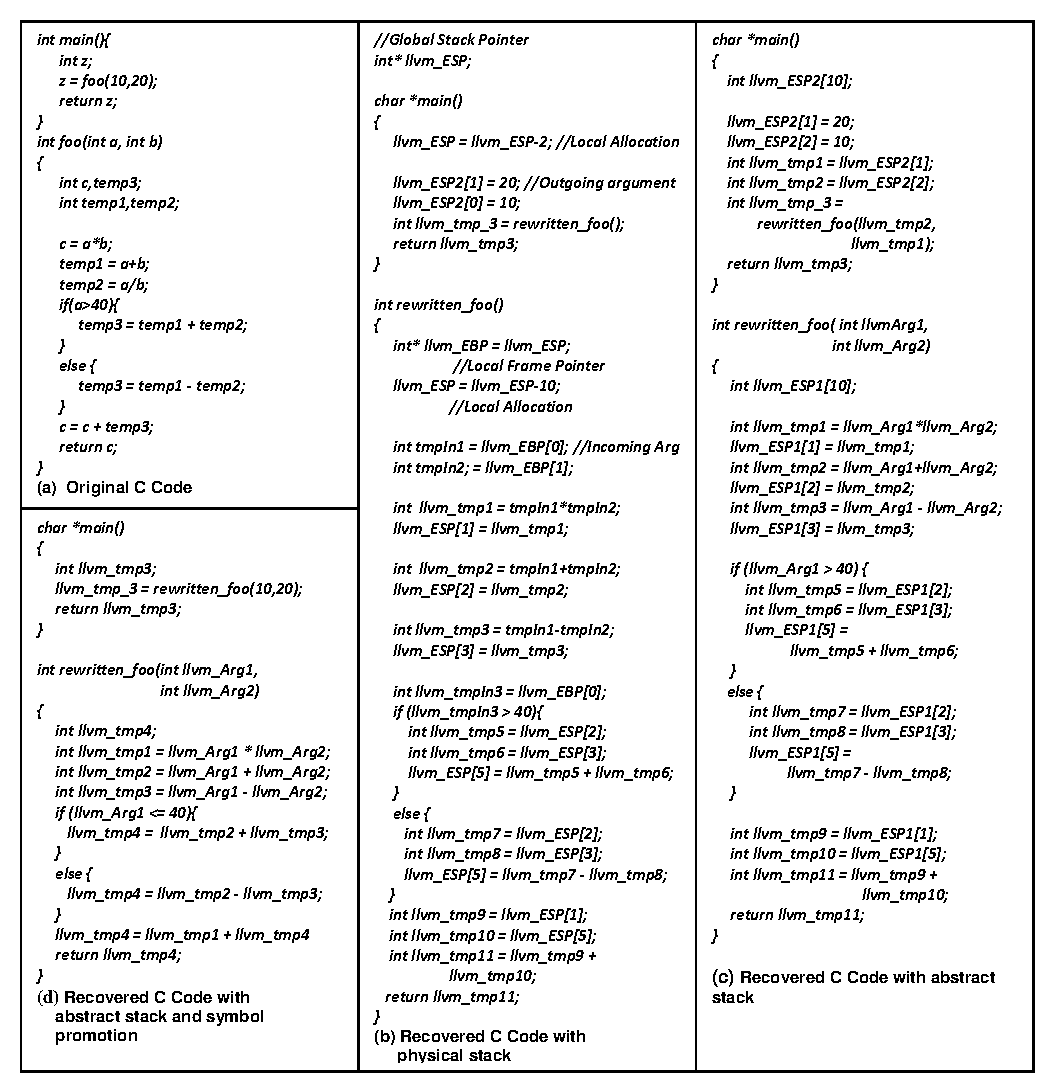
\includegraphics[width=\linewidth]{figures/EPS/c-code-example.eps}
%\vspace{-3ex}
\caption{\textit{Source Code Example}}
\label{fig:origCCode}
}
\end{minipage}
\hfill
\begin{minipage}{.40\linewidth}
\centering
{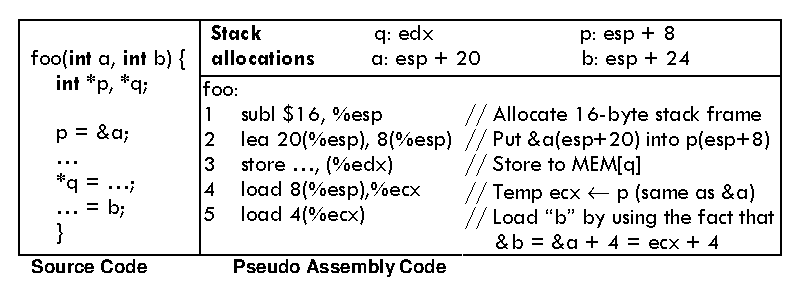
\includegraphics[width=\linewidth]{figures/EPS/abstract-stack-diff-new.eps}
\caption{\textit{An example showing the limitation of existing methods for detecting arguments}}
\label{fig:abstract-stack-diff}
}
\vspace{1ex}
{
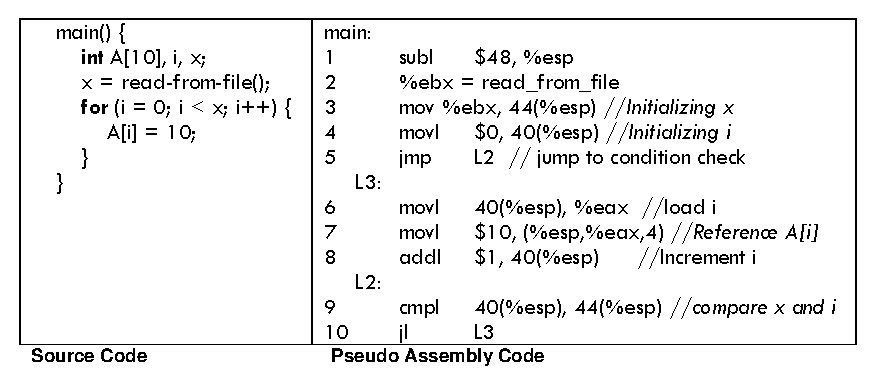
\includegraphics[width=\linewidth]{figures/EPS/new-var-prom-diff.eps}
\caption{\textit{An example showing that variable identification and symbol promotion are different}}
\label{fig:ident-prom-diff}
}
\vspace{1ex}
{
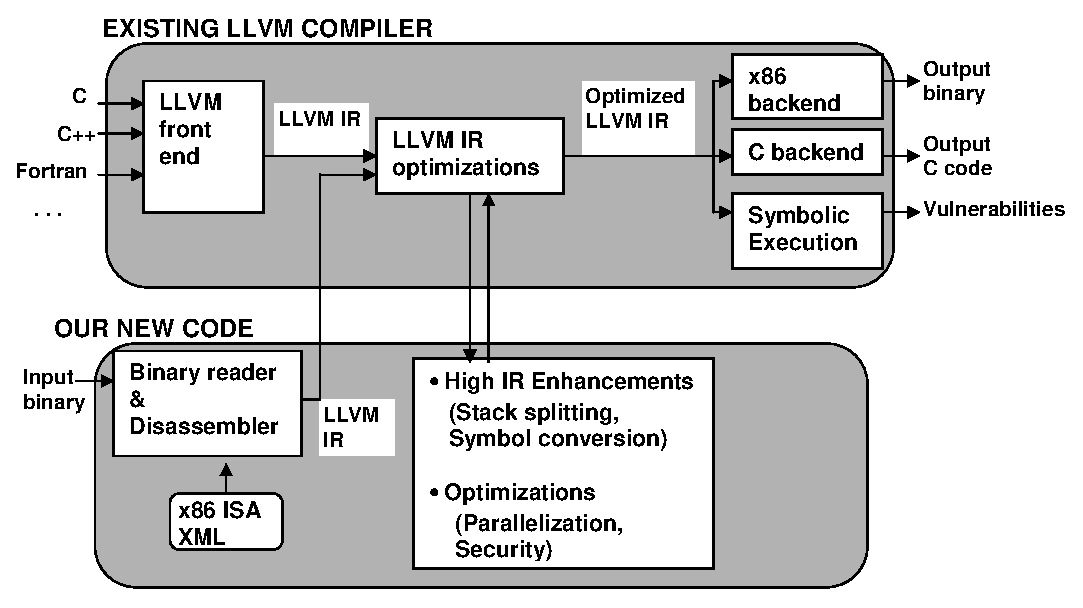
\includegraphics[width=0.8\linewidth]{figures/EPS/flow1.eps}
\caption{\textit{System Flow}}
\label{fig:systemflow}
}
\end{minipage}
%\vspace{-4ex}
}
\vspace{-1ex}
\end{figure*}

% compiler IR allows binary frameworks to leverage a substantial body of research work on source-level analysis and enables their application to binaries without any modifications.
%Our framework is designed to achieve three goals: rewritability, analyzability and understandability. present various techniques to convert a binary to a compiler intermediate representation and 
\squishlist

\item \textbf{Binary Rewriting}
Existing binary backend of the compiler is employed to obtain a new rewritten binary. The presence of a compiler-IR provides various advantages to our framework (i) It enables every complex compiler transformation like automatic parallelization and security enforcements to run on binaries without any binary-specific customization. (ii) Sharing the IR with a mature compiler allows leveraging the full set of compiler passes built up over decades by hundreds of developers. 
%Our method becomes a great enabling platform to statically optimize binaries with future optimizations by other researchers, which may not have been developed yet.  We display this application by implementing advanced source level automatic parallelization and security enforcements on binaries. 
%(iii) The presence of variables and symbols in compiler IR allows dataflow analyses to become much more effective.

%Our current binary rewriting framework is able to correctly rewrite the complete SPEC 2006 benchmark suite and some real-world programs on two different operating systems. The rewriter backend accelerates un-optimized binaries by 42\% on average, and further optimizes higly optimized (produced by gcc) binaries by 6.5\% just by using standard optimizations present in LLVM. 
% It retains the performance of binaries produced by visual studio. 

\item \textbf{Symbolic Execution} KLEE~\cite{Cadar-KLEE}, a source level symbolic execution engine, is employed directly in our framework without any modifications for detecting vulnerabilities in binaries. Various source level symbolic executors~\cite{Cadar-EXE, Cadar-KLEE} reason about symbolic memory\footnote{The symbolic memory access arises whenever the address referenced in a load or store operation is an expression derived from the user input} using logical solvers. Directly applying such source-level models to binaries results in high overhead; hence, previous symbolic execution engines for binaries~\cite{Song-Bitblaze,Chipounov-S2E} make unsound assumptions by concretizing symbolic memory accesses to a fixed location. Our techniques of obtaining a compiler IR enable simulating a fully symbolic memory using logical solvers for binaries without any excessive cost. 

%This demonstrates the ability of our frameworks to employ source level techniques directly for executables. , Brumley-BAP
%Our techniques for obtaining a compiler IR help in efficient reasoning of \emph{symbolic memory}, where the address in a memory access instruction depends on user input.

%to reason about symbolic indices
%allow an efficient extension of above source-level memory models and
%Most of the existing symbolic execution engines operating at binary level~\cite{Song-Bitblaze, Brumley-BAP} make unsound assumptions about symbolic memory indices by concretizing it to a fixed (and feasible) memory location. On the other hand,
%Further, the presence of a simultaneous rewriting and symbolic execution path provides a unique capability to our framework. It enables us to not only detect a bug in the input binary, but also fix the bug. We illustrate this interesting application by obtaining a rewritten binary after fixing a bug in IR detected using the symbolic execution.

\item \textbf{Source code recovery}
The compiler's C backend is used to convert the IR obtained from a binary to C source-code. Unlike existing tools, which do not ensure the functional correctness of the output code~\cite{boomerang, hex-rays}, our framework produces a functionally correct source code which can be updated and recompiled by any source code compiler.
% to obtain a new binary.decompilers or binary understanding 

Various organizations like the US Department of Defense(DoD)~\cite{DARPA-BET1} have  critical applications that have been developed for older systems and need to be ported to future versions. In many cases, the application source code is no longer accessible requiring these applications to continue to run on outdated configurations. The ability of our framework to recover a functionally correct source code is highly useful in such scenarios.
% for legacy binaries. 
%Further, our methods of promoting memory references to symbols in IR drastically improves the readability and the understanding of the resulting source code. 

\squishend

It is conventional wisdom that static analysis of executables is a very difficult problem, resulting in a plethora of dynamic binary frameworks. However, a static binary framework based on a compiler IR enables applications not possible in any existing tool and our results establish the feasility of this approach for most pragmatic scenarios. This work should be seen as what it is: a first successful attempt to statically recover a functional compiler IR from executables, rather than the last word. We do not claim that we have fully solved all the issues; statically handling every program in the world may still be an elusive goal. However, the resulting experience of expanding the static envelope as much as possible is a hugely valuable contribution to the community.
%is still a significant advance and hugely valuable contribution to the community.
%through the selective use of run-time checks

The rest of the paper is organized as follows. Sec~\ref{sec:contributions} highlights our contributions and describes our framework, Sec~\ref{sec:deconstructFrame} and Sec~\ref{sec:symprom} present our analyses for obtaining compiler IR. Sec~\ref{sec:symExec} presents the extensions of our analysis for symbolic execution. Sec~\ref{sec:practicalCons} discusses some practical issues regarding our framework followed by the evaluations in Sec~\ref{sec:results}.

